\newpage
\section{The Hopf-Lax Solution to Hamilton-Jacobi Equations}
\textbf{Date:} Sep 28, 2021

\subsection{The Hamiltonian in classical mechanics}
Last time, we were solving the Hamilton-Jacobi equation
$$
\left\{\begin{array}{l}
u_{t}+H(x, D u)=0 \\
u(0)=u_{0}
\end{array}\right.
$$
using the calculus of variations:
$$
u(x, t)=\inf _{y(t)=x} \int_{0}^{t} L(y(s), \dot{y}(s)) d s+u_{0}(y(0))
$$

\begin{theorem}
The function $u$ solves the Hamilton-Jacobi equation as long as the solutions the solutions stay smooth.
\end{theorem}
In the proof, we had the convex duality
$$
H(x, p)=\max _{q} p \cdot q-L(x, q)
$$
for the Hamiltonian $H(x, p)$ and the Lagrangian $L(x, q)$.

\begin{example}
    Here is an example from classical mechanics. Consider the Lagrangian
    \[
        L(x, q)=\frac{1}{2} m q^{2}-\phi(x),
    \]
    where $\frac{1}{2} m q^{2}$ is kinetic energy and $\phi(x)$ is potential energy. Then
$$
H(x, p)=\sup _{q} p \cdot q-\frac{1}{2} m q^{2}+\phi(x)
$$
Complete the square to get
$$
\begin{aligned}
&=\sup _{q} \frac{1}{2 m} p^{2}-\frac{1}{2 m}(p-m q)^{2}+\phi(x) \\
&=\frac{1}{2 m} p^{2}+\phi(x)
\end{aligned}
$$
In the physical interpretation, the Hamiltonian $H(x, p)$ plays the role of the energy of the system.
\end{example}


\subsection{The Hopf-Lax formula}
Now we will consider a special case, where $L=L(q)$ does not depend on $x$ (and consequently $H=H(p)) .$ Assume that $L, H$ are strictly convex and coercive (i.e. $\lim _{q \rightarrow \infty} \frac{L(q)}{|q|}=$ $\infty$ ). The Euler-Lagrange equation tells us that
\[
    \frac{d}{dt}L_q(y,\dot y) = 0.
\]
So we get that $L_{q}(\dot{y})$ is constant. Since $L_{q}$ is a local diffeomorphism, we get that $\dot{y}$ is constant. That is, the solutions to the Euler-Lagrange equation are linear.

We claim that fixing the endpoints $y(0), y(t)$, the minimum is attained for linear trajectories.

\begin{theorem}
    [Hopf-Lax formula] If $L=L(q)$ is convex, then 
    \[
        u(x, t)=\inf _{y} u_{0}(y)+t L\left(\frac{x-y}{t}\right).
    \]
\end{theorem}
\begin{proof}
    Since 
    \[
        int_0^t \dot y(s) \,ds = y(t) - y(0),
    \]
    we can average to get 
    \[
        \frac 1 t \int_0^t \dot y(s) \, ds = \frac{y(t)- y(0)}{t},
    \]
    where the right hand side is the average velocity for a straight path. Then 
    \[
        \int_0^t L(\dot y(s)) ds = t\cdot \frac{1}{t}\int_0^t L(\dot y(s)) ds \ge t \cdot L(\frac{y(t) -y(0)}{t}).
    \]
    In the inequality, we apply Jensen's inequality. In other owrds, the cost of an arbitrary path is larger than the cost of the straight path. 
    \qed 
\end{proof}
We are not done yet, we still have to minimize $u_0(y(0))$ over the choice of $y(0)$.

\subsection{Properties of the Hopf-Lax solution}
Assume $L$ is convex and coercive. For simplicity, also assume that $u_0$ is bounded . Observe that if $t>0$, then we can restrict $q = \frac{x-y}{t}$ to a compact set. So if $u_0$ is also continuous, then the infimum is attained.

\begin{proposition}
    If $u_0\in \Lip$, then $u \in \Lip$.
\end{proposition}

\begin{proof}
    Suppose we have points $x_1, x_2$, and $y$ such that 
    \[
        tL(\frac{x_2-y}{t})+g(y) = u(x,t).
    \]
    Then 
    \[
        \begin{aligned}
            u(x_1, t)-u(x_2, t) &=\min _{z}\left\{t L\left(\frac{x_1-z}{t}\right)+u_0(z)\right\}-t L\left(\frac{x_2-y}{t}\right)-u_0(y) \\
            & \leq u_0(x_1-x_2+y)-u_0(y) \leq \operatorname{Lip}(u_0)|x_1-x_2|
            \end{aligned}
    \]
    Interchaging the roles of $x_1,x_2$, we find 
    \[
        |u(x_1,t) - u(x_2, t) | \le \Lip(u_0)|x_1-x_2|.
    \]

    \qed 
\end{proof}

What if we don't assume $u_0$ is Lipschitz? Can we still conclude that $u$ is Lipschitz? 

\begin{proposition}
    If $u_0$ is continuous, then $u(t)$ is Lipschitz.
\end{proposition}
\begin{proof}
    In this case, we compare $x_1$ and $x_2$ to the same $y$. We have 
    \[
        \begin{aligned}
            &u\left(x_{1}\right)=\inf _{y} u_{0}(y)+tL\left(\frac{x_{1}-y}{t}\right) \\
            &u\left(x_{2}\right)=\inf _{y} u_{0}(y)+tL\left(\frac{x_{2}-y}{t}\right)
            \end{aligned}
    \]
    The difference
    \[
        \left|L\left(\frac{x_{1}-y}{t}\right)-L\left(\frac{x_{2}-y}{t}\right)\right| \leq C \cdot \frac{\left|x_{1}-x_{2}\right|}{t},
    \]
    where the Lipschitz constant $C=C(t)$ in the set where $\frac{x_1-y}{t}$ and $\frac{x_2-y}{t}$ live. 
    Where should we look? $\frac{y-x_1}{t}, \frac{y-x_2}{t}$ cannot be too large. Let $x=x_1=x_2$, and compare the straight trajectory to an arbitrary trajecotry. The oblique trajectory loses if $u_0+tL(0) \le u_0(y)+ tL(\frac{x-y}{t})$. This is when $2M/t \le L(\frac{x-y}{t})$. So we can restrict to $y$ such that $L(\frac{x-y}{t})\le 2M/t$. So $\frac{x-y}{t}$ is in a compact set depending on $t$. Then the conclusion is that 
    $$
\left|u\left(x_{1}, t\right)-u\left(x_{2}, t\right)\right| \leq C(t) \cdot \frac{\left|x_{1}-x_{2}\right|}{t}
$$
where $C(t)$ is the Lipschitz constant for $L$ in the region $L(q) \leq \frac{C}{t} .$ This Lipschitz constant goes to $\infty$ as $t \rightarrow 0$. \qed 
\end{proof}

In terms of the Hamilton-Jacobi equation, there will be lots of velocities with different speeds. So there is only an average velocity that survives. We say that this PDE has a mild \textbf{regularizing effect}.
\wc{Ask about the proof and the regularizing effect}

\subsection{Almost everywhere solvability of the H-J equation}
\begin{theorem}
    If $u$ is a Lipschitz function, then $u$ is differentiable almost everywhere.
\end{theorem}
\begin{corollary}
    The solution $u$ is differentiable almost everywhere.
\end{corollary}

\begin{proposition}
    Let $(x,t)$ be a differentiable point for $u$. Then the H-J equation hold at $(x,t)$.
\end{proposition}

\begin{corollary}
    The function $u$ solves the H-J equation almost everywhere. 
\end{corollary}

Let's prove the proposition first. 
\begin{proof}
    We can think of the Hamilton-Jacobi equation as proving two separate inequalities.
    If our trajectory is optimal, then it is optimal if we only look at the trajectory at a shorter length of time. Look at the optimal trajectory, ending at $y$ and with slope $\frac{x-y}{t}$.
    Then,
$$
u(x, t)=u_{0}(y)+t L\left(\frac{x-y}{t}\right)
$$
so
$$
u\left(x-h \frac{x-y}{t}, t-h\right)=u_{0}(y)+(t-h) L\left(\frac{x-y}{t}\right)
$$
The first equation tells us that $y$ is the optimal trajectory for $(x, t)$, and the second says that $y$ is optimal for $\left(x \cdot h \frac{x-y}{t}, t-h\right)$. Let $q=\frac{x-y}{t}$. Then dividing by $h$ gives
$$
\frac{u(x, t)-u(x-h q, t-h)}{h}=h L(q)
$$
Letting $h \rightarrow 0$ gives
$$
\partial_{x} u \cdot q+\partial_{t} u=L(q)
$$
So for this special $q$ we have chosen,
$$
\partial_{t} u+\partial_{x} u \cdot q-L(q)=0
$$
We want to think of this in terms of the Legendre transform. Since $H(p)=\sup p \cdot q-L(q)$, the latter half of our equation, $\partial_{x} u \cdot q-L(q)$, is $\leq H\left(\partial_{x} u\right) .$ So we get
$$
\partial_{t} u+H\left(\partial_{x} u\right) \geq 0
$$
Now we want to produce the other inequality. Notice that for the previous inequality, it was enough to work with a specific value of $q$, whereas for this direction, we will need to look at all values of $q$. Instead of looking at the past of $(t, x)$, look at the future of $(t, x)$. Our trajectory looks like 

\begin{figure}[H]
    \centering
    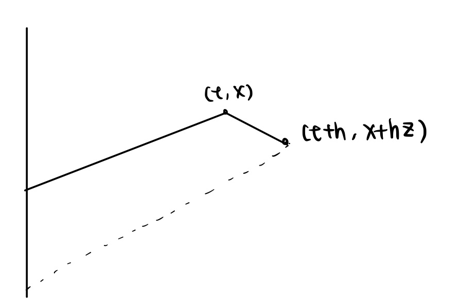
\includegraphics[width=0.7\textwidth]{pics/10-1.png}
\end{figure}

One trajectory from $(t+h, x+hz)$ is to go through $x$, but this may not be optimal. So 
\[
    u(t+h,x+hz)\le u(t,x) + \underbrace{hL(z)}_{\int_t^{t+h} L(z) ds}
\]
As before, subtract the right hand side, divide by $h$ and let $h\to 0$. Then we get 
\[
    \frac{u(t+h, x+h z)-u(t, x)}{h} \leq L(t) \Longrightarrow \partial u+\partial_{x} u z \leq L(z).  
\]
So we have proven that for all $z$,
\[
    \partial_{t} u+\partial_{x} u \cdot z -L(z)\leq 0.
\]
Taking the supremum over all $z$, we get 
\[
    \partial_{t} u+H\left(\partial_{x} u\right) \leq 0.
\]
\qed 
\end{proof}

Now we will tell a story. The details are in Evans' book, but the overall story is more important. We want to ask a question: Does solving the Hamilton-Jacobi equation almost everywhere suffice to guarantee uniqueness for Hamilton-Jacobi? Equivalently, does this guarantee that $u$ is the minimal value function? The answer is no.

Are there other interesting properties for the function $u$ ? Look at the Hopf-Lax formula
$$
u(x, t)=\inf_y u_{0}(y)+t L\left(\frac{x-y}{t}\right)
$$
Observe that this is an infimum of functions which are smooth in $x$. We can compare what this looks like for different optimal/nonoptimal $y$:

\begin{figure}[H]
    \centering
    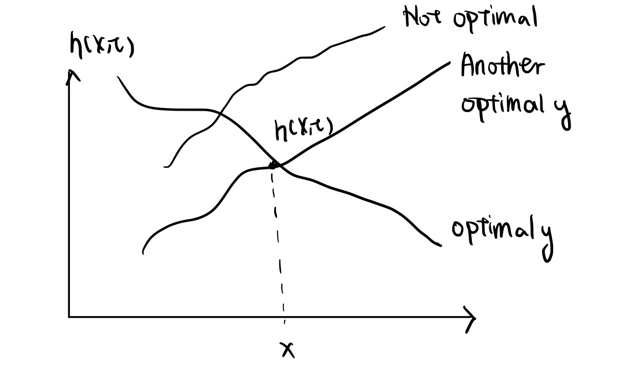
\includegraphics[width=0.7\textwidth]{pics/10-2.png}
\end{figure}

Since we are taking a minimum, we can see that our curve could ave a corner pointing upwards, but a conner pointing downwards is not possible. This points to a concavity property of our solution.

\begin{proposition}
    $u$ is semiconcave.
\end{proposition}
Concave means that $u(t, x) \geq \frac{u(t, x+y)+u(t, x-y)}{2} .$ \textbf{Semiconcave} means that
$$
u(t, x) \geq \frac{u(t, x+y)+u(t, x-y)}{2}-c \cdot|x-y|^{2}.
$$

\begin{theorem}
    The optimal value function $u$ is the unique seminconcave solution to the H-J equation.
\end{theorem}
The proof is in Evans, but it is a little hard to follow. There is a better way to do things! Instead of plugging in $u$ to check whether it satisfies the equation, if we have a corner, draw a tangent test function $\varphi$ with $\varphi_{t}+H\left(\partial_{x} \phi\right) \geq 0$ or $\varphi_{t}+H\left(\partial_{x} \phi\right) \leq 0$.

\begin{figure}[H]
    \centering
    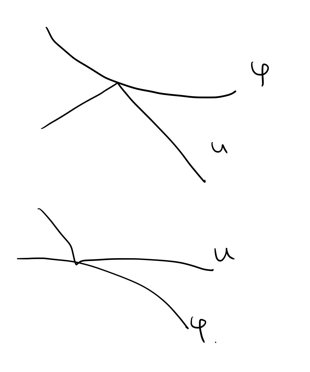
\includegraphics[width=0.6\textwidth]{pics/10-3.png}
\end{figure}

These are called \textbf{viscosity solutions} for H-J equations.
